\documentclass{article}


% if you need to pass options to natbib, use, e.g.:
    \PassOptionsToPackage{numbers, compress}{natbib}
% before loading neurips_2024


% ready for submission
% \usepackage{neurips_2024}


% to compile a preprint version, e.g., for submission to arXiv, add add the
% [preprint] option:
% \usepackage[preprint]{neurips_2024}


% to compile a camera-ready version, add the [final] option, e.g.:
\usepackage[final]{neurips_2025}


% to avoid loading the natbib package, add option nonatbib:
% \usepackage[nonatbib]{neurips_2024}


\usepackage[utf8]{inputenc} % allow utf-8 input
\usepackage[T1]{fontenc}    % use 8-bit T1 fonts
\usepackage{hyperref}       % hyperlinks
\usepackage{url}            % simple URL typesetting
\usepackage{booktabs}       % professional-quality tables
\usepackage{amsfonts}       % blackboard math symbols
\usepackage{nicefrac}       % compact symbols for 1/2, etc.
\usepackage{microtype}      % microtypography
\usepackage{xcolor}         % colors
\usepackage{amsmath}
\usepackage{graphicx}
\usepackage{array}
\usepackage{multirow}
\usepackage{float} 
\usepackage{ctex}

\hypersetup{colorlinks=true,linktoc=all}

%%%%%%%%%%%%%%%%%%
% \title{DeTeCtive: \underline{De}tecting AI-generated \underline{Te}xt from \\ a \underline{C}ontras\underline{tive} Perspective}

\title{高算力芯片专题调研报告}

% The \author macro works with any number of authors. There are two commands
% used to separate the names and addresses of multiple authors: \And and \AND.
%
% Using \And between authors leaves it to LaTeX to determine where to break the
% lines. Using \AND forces a line break at that point. So, if LaTeX puts 3 of 4
% authors names on the first line, and the last on the second line, try using
% \AND instead of \And before the third author name.

\newcommand*\samethanks[1][\value{footnote}]{\footnotemark[#1]}
\author{%
  \textbf{杨枭\textsuperscript{1}} 
 \\
  2022211286\textsuperscript{1} 
  \\
  \texttt{yangxiao@bupt.edu.cn} 
}

\begin{document}  
\maketitle
\begin{abstract}
  随着人工智能、大数据和云计算技术的爆发式增长，算力芯片作为支撑智能时代的核心硬件，其研发与应用已成为全球科技竞争的战略制高点\cite{hager2010introduction}。当前主流算力芯片以GPU（图形处理器）、NPU（神经网络处理器）和TPU（张量处理器）为代表，通过并行计算架构创新实现算力跃升\cite{hager2016exploring}。其中，GPU凭借高通用性和成熟的软件生态占据主导地位，而TPU、NPU等专用芯片则通过算法与硬件协同优化，在能效比和场景适配性上展现优势。从市场格局看，国际巨头英伟达、谷歌、英特尔通过软硬协同构筑技术壁垒，而中国企业在政策扶持下加速国产替代进程，华为昇腾、寒武纪等企业已在AI芯片领域实现突破，但高端制程依赖和生态短板仍是主要挑战。未来，随着大模型算力需求激增，并行架构创新、先进制程以及绿色化、标准化的良性准则或将成为技术突破方向，而产业链自主可控与全球化竞争将重塑行业格局。我将调研过程梳理为总体概述、常见评估指标、主流公司、高算力芯片发展、我国AI芯片现状、整体未来发展趋势六个板块，以期能对今后相关方向上自己亦或是他人的工作带来参考，本次调研的所有材料及写作见\url{https://github.com/simonsshoot?tab=repositories}。
\end{abstract}

\section{引言与概述}
在数字经济与智能化浪潮的深刻变革中，算力已成为驱动科技革命的核心引擎\cite{yao2022high}。全球算力需求正以年均30\%的速度激增，其中，人工智能大模型（如GPT-4\cite{achiam2023gpt}、DeepSeek\cite{liu2024deepseek}等）的参数量已突破万亿级，单次训练所需的浮点运算量较十年前增长超10万倍。传统通用处理器（CPU）则因能效比低、并行处理能力不足等缺陷，难以支撑AI训练、自动驾驶、科学仿真等高密度计算场景的需求\cite{hager2016exploring}。在此背景下，高算力芯片（GPU、NPU、TPU等）凭借其专用化架构与硬件级优化，成为人工智能、云计算、边缘计算等领域的核心硬件基石。

当前，高算力芯片的技术发展已从“堆砌算力”转向“效能跃迁”。存算一体技术通过打破“内存墙”限制\cite{melnyk2016parallel}，将计算与存储深度融合，清华大学研发的忆阻器存算一体芯片能效比达传统GPU的100倍；Chiplet异构集成通过模块化组合提升算力密度，如AMD MI300X集成1460亿晶体管，算力密度较单片设计提升3倍\cite{shan2022architecture,naffziger2020amdchiplet,narashiman2024chiplets}；光子计算则以超低功耗路径探索未来，Lightmatter的光子芯片推理速度较传统GPU快10倍。同时，先进制程工艺向3nm及以下节点突破，晶体管密度突破千亿级，华为昇腾910B等国产芯片已基于7nm工艺实现256 Tera-FLOPS的算力突破\cite{lee2024huawei}。

市场层面，全球高算力芯片呈现“双轨并行”特征。国际巨头如英伟达凭借H100（4nm制程）和CUDA生态占据云端训练市场90\%份额，谷歌TPUv4超算集群算力达1.1 ExaFLOPS。中国则在政策驱动下加速国产替代，2024年国产芯片在数据中心的中标率超70\%，华为昇腾、寒武纪等企业逐步突破技术壁垒\cite{lee2024huawei}。然而，供应链依赖（如7nm以下制程需台积电代工）与生态壁垒（CUDA生态垄断）仍是主要挑战。

未来，高算力芯片的竞争将聚焦异构计算与架构创新（CPU+GPU+NPU协同，存算一体打破内存墙限制）、开源生态（RISC-V架构降低开发门槛）与绿色计算（液冷散热、能效优化）等方面展开。此外，先进制程如光子计算、量子融合等颠覆性技术或重构算力范式。从我国芯片发展角度而言，国产芯片需通过架构创新与产业链协同，在大模型大数据时代下抢占市场机遇，在高算力日趋重要的背景下果断力争上游，在“东数西算”等国家战略下实现自主可控。这份报告，也是自己在高算力芯片领域，从零开始，逐步调研，逐步深入的过程和记录，将系统解析高算力芯片的技术路径、市场格局与未来趋势等方面，为中国在全球算力革命中抢占战略高地提供自己的洞察。

\begin{figure*}[h]
  \centering
  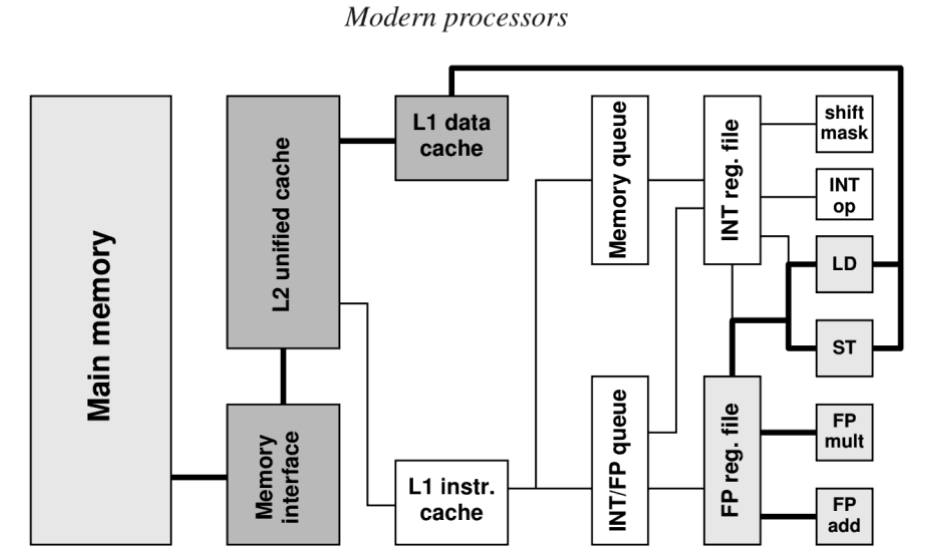
\includegraphics[width=0.9\textwidth]{pics/modern_processor.png}
  \caption{现代处理器架构}
\end{figure*}

\section{常见评估指标}
一般而言，可将衡量高算力芯片的指标分为算力指标（FLOPS、TOPS）、功耗指标、实时性指标等\cite{yao2022high}。
\begin{equation}
	\label{eq:metric_OPS}
	FLOPS=\frac{\text{浮点运算次数}}{\text{时间（秒）}}\quad TOPS=\frac{\text{整数运算次数}}{10^{12}\text{时间（秒）}}
\end{equation}
$FLOPS$：每秒浮点运算次数，衡量芯片的浮点计算能力，支持不同精度（如FP16、FP32、FP64），FP16混合精度下的FLOPS值对AI训练尤为重要。

$TOPS$：每秒万亿次整数运算次数，衡量芯片的整数计算能力，支持不同精度（如INT8、INT16、INT32），适用于AI推理场景。
\begin{equation}
  \label{eq:metric_comsuption}
  \eta=\frac{FLOPS}{W} \quad P_{dynamic}=\alpha\times C \times V^2 \times f
\end{equation}
$\eta$：性能功耗比，又称能效比，衡量单位功耗下的算力输出。

$P_{dynamic}$：动态功耗，由晶体管开关产生，与电压和频率相关。其中，$\alpha$为电压因子，$C$为芯片的容量，$V$为电压，$f$为频率。
\begin{equation}
	\label{eq:metric_total}
	% 芯片总算力公式
\text{总算力} = \gamma \times \left( \frac{M_{\text{TOPS}}}{N} \right) \times \left( \frac{N}{S} \right) \times S
\end{equation}
$\gamma$:互连系数（$\leq0\leq\gamma\leq1$），表征数据互连效率，包括存储与计算单元之间、计算单元之间的带宽利用率。
$M_{\text{TOPS}}$:以TOPS（每秒万亿次操作）为单位的单位晶体管算力，由芯片架构（如并行度、指令集）决定。
$N$:芯片中晶体管的总数量，与制程工艺（如3nm、5nm）和晶体管密度相关。
$S$:芯片物理面积。受制造工艺和封装技术限制。
\section{主流公司}
\paragraph{英伟达NVIDIA.}
作为全球AI计算领域的领导者，英伟达以CUDA软件生态和GPU架构创新构建技术壁垒。其最新Blackwell架构\footnote{\url{https://resources.nvidia.com/en-us-blackwell-architecture}}采用4nm制程，集成Transformer引擎和第三代NVLink技术，支持多精度计算（FP16/INT8/FP4）和多GPU高速互联，显存带宽高达3.35 TB/s\cite{tirumala2024nvidia}。代表产品如H100（FP16算力67.8 TFLOPS）和GB200（FP16算力5000 TFLOPS）专为千亿参数大模型训练设计，覆盖数据中心、自动驾驶（如DRIVE Hyperion平台）等场景。此外，英伟达通过Omniverse平台布局元宇宙，推动虚拟与现实融合的工业仿真应用\cite{hummel2019leveraging,vatanen2024exploring}。
\paragraph{超威半导体AMD.}
AMD凭借Chiplet异构集成技术和Zen架构在CPU/GPU市场双线突破\cite{schone2021energy}。其MI300系列数据中心GPU采用5nm制程，集成CPU与GPU模块，FP16算力达153 TFLOPS，支持AI与科学计算的融合场景。EPYC霄龙服务器处理器和Instinct加速器（如MI325X）则通过Infinity Fabric互联提升并行效率，对标英伟达H系列。消费级产品如锐龙（Ryzen）处理器和Radeon RX显卡则通过RDNA 3架构优化能效比，抢占游戏与边缘计算市场。
\paragraph{谷歌Google.}
谷歌自研TPU（Tensor Processing Unit）专为AI优化，最新TPU v7p（Ironwood）采用3nm制程，晶体管密度308百万/mm²，FP16算力2307 TFLOPS，支持万亿参数模型训练\cite{kumar2019scale}。其架构针对Transformer模型设计，结合TensorFlow框架实现软硬协同优化，显著提升能效比。谷歌还通过Gemini大模型和量子计算研究，推动AI与量子技术融合。此外，Chrome浏览器与Android系统的高效适配进一步巩固其生态优势。
\paragraph{英特尔Intel.}
英特尔正从传统CPU向异构计算转型，Gaudi 3 AI加速器采用5nm制程，FP16算力1835 TFLOPS，支持主流AI框架\cite{zhang2023benchmarking}。其IDM 2.0战略整合先进封装（如EMIB）与制程技术（Intel 20A），布局AI芯片、自动驾驶（Mobileye）及量子计算。至强（Xeon）处理器和Arc GPU通过OneAPI工具链实现跨平台开发，覆盖数据中心与边缘端。近期推出的Core Ultra处理器集成NPU模块，强化PC端AI推理能力。

\begin{figure*}
  \centering
  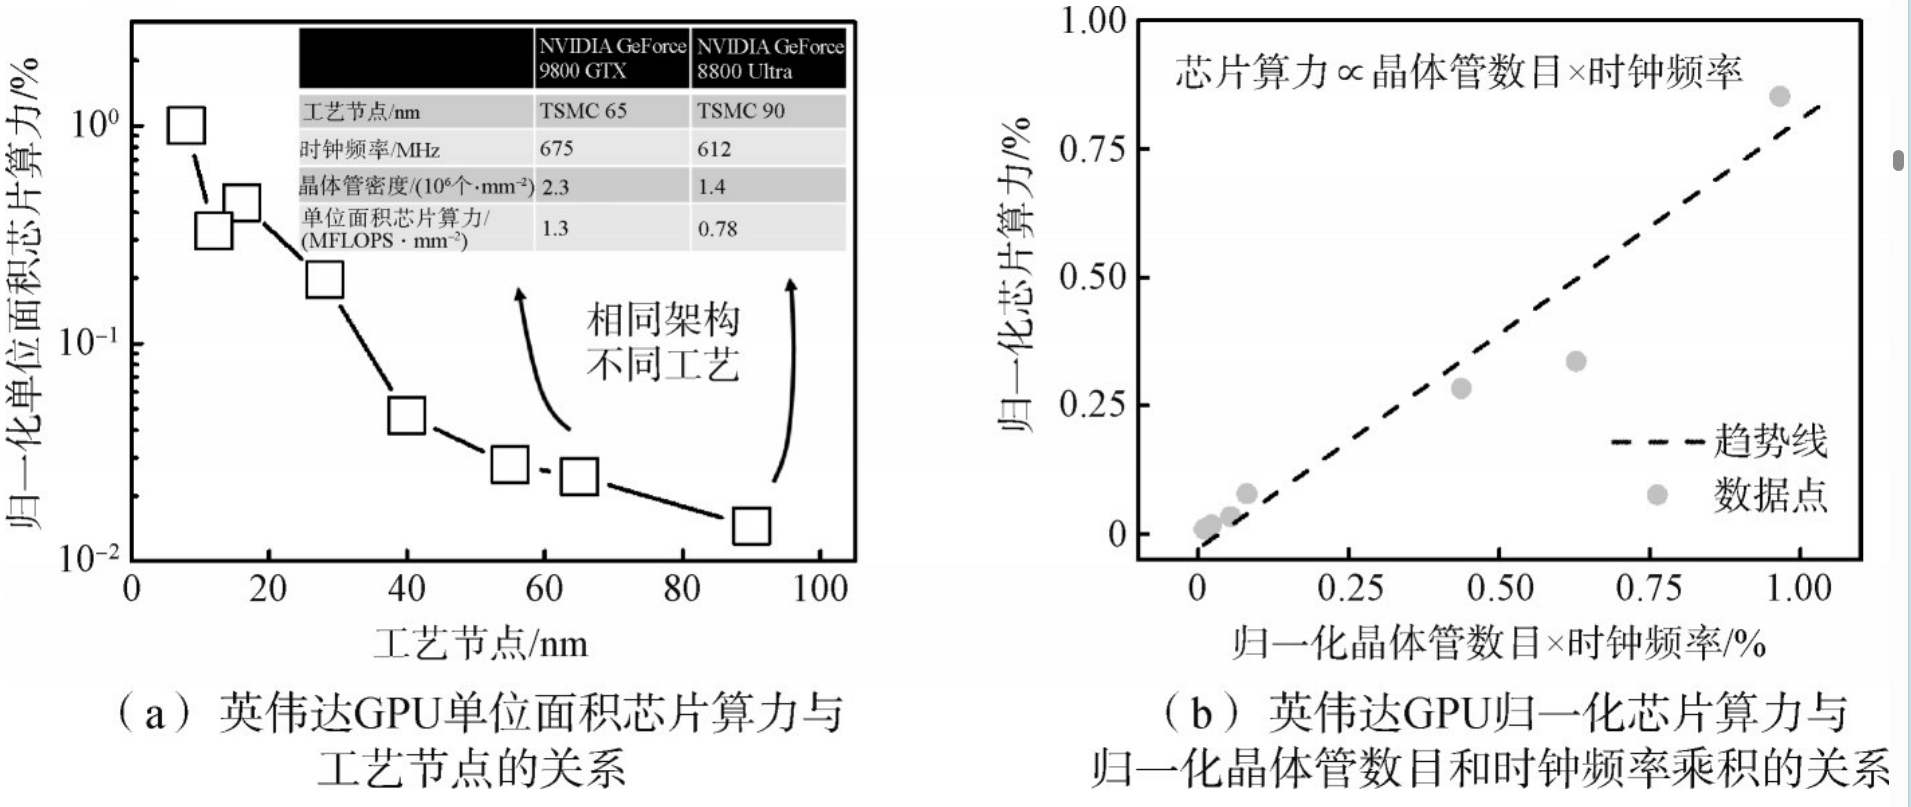
\includegraphics[width=0.9\textwidth]{pics/chip_power.png}
  \caption{芯片算力影响因子}
\end{figure*}
\section{高算力芯片发展}
高算力芯片的发展经历了从GPU到NPU再到TPU的演进过程。GPU最初专为图形渲染设计，2006年NVIDIA推出CUDA架构后，其并行计算能力被拓展至科学计算和AI领域，成为深度学习训练的核心硬件。NPU则诞生于2010年代深度学习爆发期，专为神经网络优化，2017年苹果率先在手机芯片中集成NPU（如A11仿生芯片），随后华为、高通等厂商跟进，使其在移动端图像识别、语音处理等场景实现低功耗实时计算\footnote{\url{https://www.szw.org.cn/20250205/68888.html}}。TPU由谷歌2016年推出，专为张量运算设计，采用脉动阵列架构，在同等制程下性能可达GPU的3-5倍\cite{kimm2021performance}，尤其适合超大规模模型训练（如AlphaGo和谷歌Gemini）\cite{norrie2021design}，中昊芯英等企业也推出类似架构芯片（如“刹那®”）\footnote{\url{https://www.huxiu.com/article/3279788.html}}，通过高速片间互联技术实现千卡集群的高效协同。
\subsection{GPU}
GPU核心架构由大量小型流处理器（如NVIDIA的CUDA核心或AMD的流处理器）组成，支持高度并行计算\cite{tirumala2024nvidia}。每个流处理器包含整数和浮点运算单元，并通过共享内存、全局内存等多层次存储系统优化数据访问效率。GPU的工作原理基于数据并行性，将任务分解为多个线程块，由流多处理器（SM）同时执行，利用流水线架构提升处理速度。  

GPU的发展历程经历了多个关键阶段，从最初的图形加速卡逐步演变为高性能并行计算的核心硬件。20世纪80年代，IBM推出的MDA和CGA等图形适配器仅负责显示，图形处理仍依赖CPU。1999年，NVIDIA发布GeForce 256\cite{dally2021evolution}，首次引入硬件变换和光照（T\&L）功能，标志着GPU作为独立图形处理器的诞生。2001年，微软DirectX 8提出顶点着色器和像素着色器概念，GPU进入可编程的Shader时代，取代了固定管线架构。2005年，ATI在Xbox 360中采用首款统一渲染架构Xenos，随后NVIDIA于2006年推出GeForce 8800 GTX（G80）\cite{fujimoto2008faster}，彻底实现统一渲染着色器，极大提升了资源利用率。与此同时，CUDA的发布为GPU通用计算奠定了基础，2011年Tesla计算卡的独立产品线确立GPU在科学计算和AI领域的主导地位。

GPU的应用场景广泛且多样化：在游戏和影视制作中，它提供高逼真渲染和实时特效支持；在人工智能领域，其并行计算能力加速深度学习模型的训练与推理；此外，GPU还用于区块链哈希运算、自动驾驶环境感知、科学模拟（如分子动力学和气象预测）以及云计算数据中心的高性能计算任务。近年来，国产GPU厂商在图形渲染和高性能计算领域持续突破，逐步缩小与国际领先技术的差距\cite{lee2024huawei}。

\subsection{NPU}
NPU（神经网络处理器）采用高度定制化架构，专为加速深度学习计算设计。其核心模块包括矩阵乘法单元（MMU）和卷积加速器，通过硬件级优化支持张量运算、激活函数（如ReLU/Sigmoid）等神经网络核心操作。内存系统采用分层设计，包含权重缓存（存储模型参数）、数据缓存（输入/中间结果）和共享内存（跨计算单元交互），显著减少外部访问延迟。控制单元则整合任务调度器和指令解码器，动态分配资源并转换AI模型为硬件指令，同时支持异构接口（如DDR5/HBM3）与CPU/GPU协同工作。

NPU的演进始于2011年谷歌提出TPU概念，2016年商用化破冰（如寒武纪终端芯片、苹果A11神经引擎）\cite{kimm2021performance}。2019年后进入技术爆发期，特斯拉Dojo芯片实现自动驾驶全流程加速，昇腾910B突破云端训练瓶颈。2023年起，3nm工艺和Chiplet技术推动算力跃升（如英伟达Grace Hopper集群），同时RISC-V开源架构降低开发门槛，NPU逐步从移动端扩展至边缘计算与云端。未来趋势聚焦光电融合计算（带宽提升10倍）、神经形态芯片（模拟生物神经元）和存算一体架构（突破内存墙限制）\cite{huang2020memory}。

NPU同样在各个领域中应用广泛。在移动设备领域，华为麒麟芯片实现实时4K影像AI降噪，高通Hexagon支持端侧70亿参数大模型运行；在自动驾驶领域，特斯拉FSD芯片完成毫秒级环境感知，地平线征程5支持L4级决策规划；在云端训练方面，谷歌TPUv5集群支撑千亿参数大模型（如Gemini），寒武纪MLU系列加速分布式训练。NPU的能效比（INT8达5TOPS/W）和低延迟（端侧语音唤醒<100ms）远超传统CPU/GPU，成为AI落地的核心硬件基石\cite{kimm2021performance}。

\subsection{TPU}
TPU（张量处理器）采用脉动阵列架构，核心模块为256×256规模的矩阵乘法单元（MXU），每个周期可执行65,536次乘加操作，专为深度学习中的张量运算优化。其内存系统集成高带宽内存（HBM），支持1.2TB/s的数据传输速率，结合片上缓存（如TPUv4的32GB HBM2E）减少数据搬运延迟。控制单元通过XLA编译器与TensorFlow框架深度协同，实现计算流水线的动态优化，同时支持低精度计算（INT8/BF16）和稀疏加速技术，能效比达同期GPU的3-5倍。

TPU的演进始于2015年谷歌为AlphaGo设计的初代TPUv1（专攻推理）\cite{norrie2021design}，2017年TPUv2/v3支持浮点运算并构建超算集群（TPUv3 Pod算力达126 PFLOPS）。2021年发布的TPUv4采用7nm工艺，算力较v3提升2.7倍，液冷技术解决高功耗问题；2025年Edge TPU扩展至边缘端（如Pixel手机实时AI摄影），同时光子计算与存算一体技术突破内存瓶颈。

TPU同样应用广泛，在云端训练领域支撑千亿参数大模型（如GPT-3、Gemini），自动驾驶中助力Waymo生成数百万虚拟驾驶场景，医疗领域加速MRI影像分割（梅奥诊所处理时间从30分钟缩短至2分钟）\footnote{\url{https://www.linngd.com/8145.html}}。其确定性计算特性（延迟可预测）和集群扩展能力（TPUv4 Pod算力突破1.1 ExaFLOPS），使其成为AI基础设施的核心硬件。

\begin{figure*} [h]
  \centering
  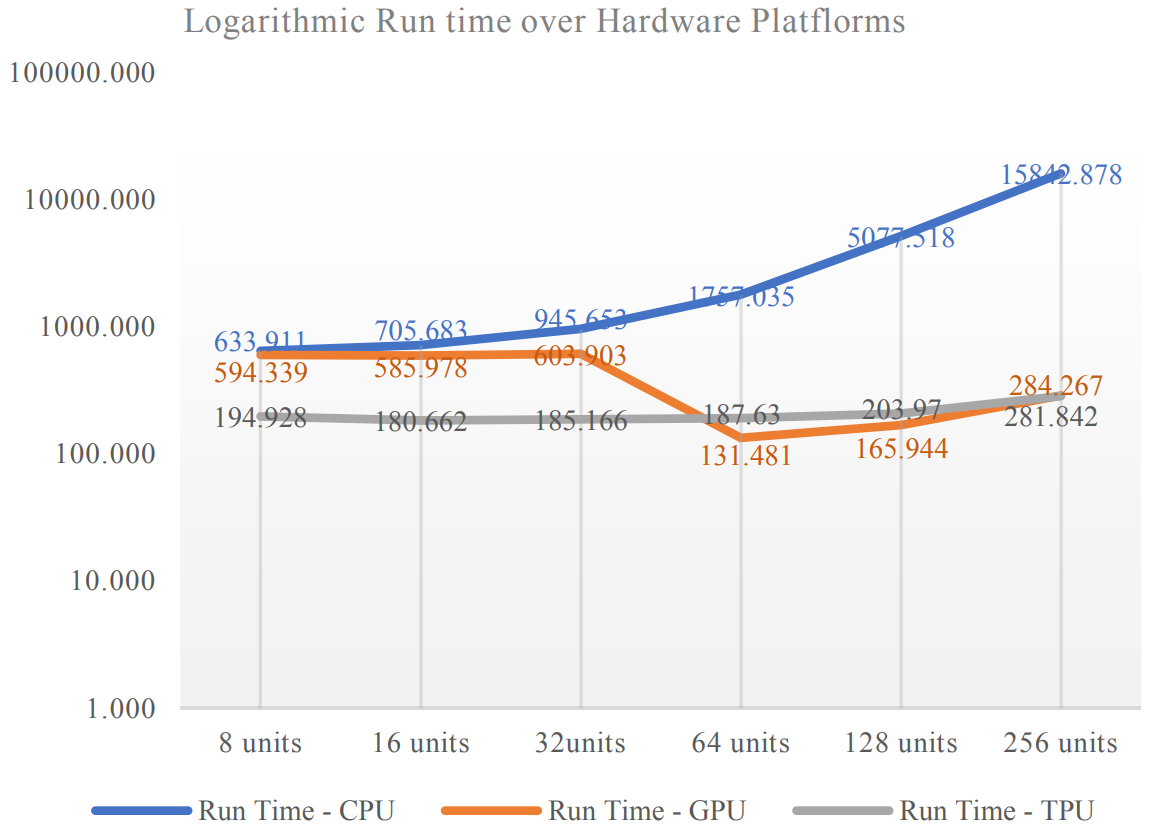
\includegraphics[width=0.9\textwidth]{pics/run_time.png}
  \caption{三大高算力芯片的时间性能对比}
\end{figure*}


% \begin{figure} [H]
%   \centering
%   \includegraphics[width=0.6\textwidth]{pics/7.png}
%   \caption{LSTM结构图}
% \end{figure}

% \begin{figure}[htbp]
%     \centering
%     \begin{minipage}[b]{0.45\textwidth}
%       \includegraphics[width=\textwidth]{pics/4.png}
%       \caption{互电容触摸感应原理}
%       \label{fig:img4}
%     \end{minipage}
%     \hfill
%     \begin{minipage}[b]{0.45\textwidth}
%       \includegraphics[width=\textwidth]{pics/3.png}
%       \caption{常见的触摸连接器接线}
%       \label{fig:img2}
%     \end{minipage}
%   \end{figure}


\section{我国高算力芯片现状}
我国AI芯片产业在核心技术攻关与产业链协同上取得显著进展。在芯片设计领域，国产企业已推出多款具备国际竞争力的产品：华为昇腾910B基于7nm+EUV工艺，FP16算力达256 Tera-FLOPS，能效比超越英伟达A100\cite{tang2025cube}；寒武纪思元590芯片针对千亿参数大模型训练优化，性能较通用GPU提升3倍。制造环节，中芯国际联合中科院开发的Chiplet技术使良品率提升至92\%，逐步缩小7nm及以下制程的工艺差距。封装测试领域，江苏长电科技的扇出型封装（FO-WLP）技术已实现量产，支持高集成度AI芯片需求。此外，新兴技术如存算一体（能效提升8倍）、光子计算（功耗仅为传统芯片1/50）进入商业化阶段，曦智科技第二代硅光AI芯片实现每秒100万亿次操作。

政策支持成为国产AI芯片发展的核心推力\cite{wei2023data}。《新一代人工智能发展规划》\footnote{\url{https://www.gov.cn/zhengce/content/2017-07/20/content_5211996.htm}}明确提出2025年国产芯片需满足70\%国内需求，长三角、粤港澳建成3个国家级AI芯片创新中心，累计投入研发资金超80亿元。市场层面，2025年我国AI芯片市场规模预计突破1530亿元，其中云端训练芯片占比45\%，边缘计算芯片增速最快（年均35\%）。应用场景多元化趋势显著：智能驾驶领域，地平线征程6芯片获6家头部车企定点，算力达128TOPS；工业质检场景中，AMD XDNA架构推理芯片将效率提升30倍。国产替代进程加速，英伟达在中国数据中心训练芯片市场份额从2022年的90\%降至2025年的65\%，华为昇腾910B在2024年国产替代项目中中标率达73\%\cite{lee2024huawei}。

尽管进步显著，国产AI芯片仍面临多重挑战\cite{wei2023data,yao2022high}。技术层面，高端制程依赖进口设备，7nm以下工艺落后国际两代；生态建设方面，英伟达CUDA生态垄断导致国产芯片需自建生态或兼容开源框架，软件适配周期长、性能差距明显。人才短缺问题突出，AI芯片领域技术人才供需比仅0.32，且高端复合型人才流失严重。未来，产业将聚焦三大方向：一是架构创新，如类脑芯片（灵汐科技LPU延迟降低90\%）\cite{moon2024lpu}和异构计算；二是工艺突破，3nm GAA工艺预计2026年量产；三是生态协同，通过开源平台（如华为昇腾社区接入17家国产芯片企业）加速技术迭代。此外，美国出口管制升级与低端同质化竞争仍是主要风险，2025年预计30\%初创企业面临并购重组。

\begin{figure*}[h]
  \centering
  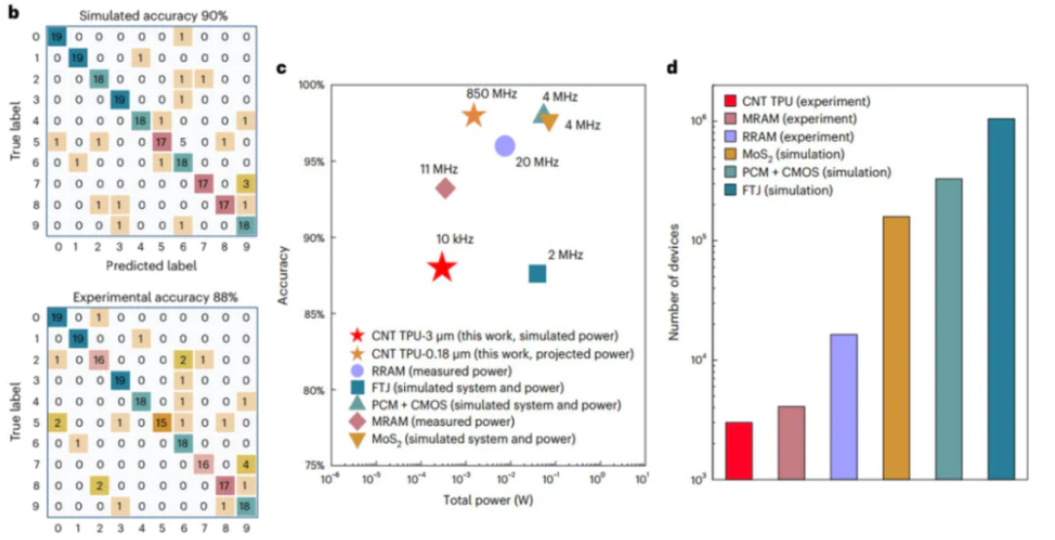
\includegraphics[width=0.9\textwidth]{pics/compare_with_nvidia.png}
  \caption{国产芯片“围攻”英伟达\protect\footnote{\url{https://www.huxiu.com/article/3279788.html}}}
\end{figure*}


\section{整体未来发展趋势}
高算力芯片的未来发展将围绕架构创新、先进制程、绿色化与标准化等方面展开\cite{wei2023data,yao2022high}。在架构层面，存算一体技术通过减少数据搬运能耗打破“内存墙”限制，例如知存科技的WTM2101芯片能效比提升10倍；Chiplet异构集成技术（如AMD MI300X\cite{naffziger2020amdchiplet}）通过小芯片组合提升算力密度并降低成本，预计2025年后3nm工艺将推动晶体管密度突破千亿级\cite{li2020chiplet}。同时，光计算芯片（如Lightmatter Envise）利用光子矩阵实现超低功耗推理，速度比传统GPU快10倍，成为千亿参数大模型的新选择\cite{gong2023nanoscale}。量子计算与类脑芯片的探索也在加速，IBM的127量子位芯片和曦智科技的“PACE”光子芯片分别代表不同技术路径的突破。此外，RISC-V开源生态的崛起降低了开发门槛，推动国产芯片在定制化领域的创新。

高算力芯片市场需求呈现全场景爆发态势\cite{zhang2024big}。在自动驾驶领域，城市NOA对算力的需求已跃升至500-1000TOPS区间，英伟达Thor芯片（2000TOPS）瞄准L4级自动驾驶；数据中心领域，2025年全球市场规模预计突破1.7万亿美元，中国占比将达35\%。国产芯片厂商如华为昇腾910B（256Tera-FLOPS）和寒武纪MLU370-X8在云端训练市场逐步替代英伟达A100，2024年国产芯片在数据中心的中标率已超70\%。政策层面，《新一代人工智能发展规划》提出2025年国产芯片自给率超70\%，长三角和粤港澳的三大创新中心累计投入研发资金超80亿元。然而，国际巨头仍主导高端市场，英伟达凭借H100（4nm制程）和CUDA生态占据38.6\%的智驾芯片份额，而国内在7nm以下先进制程仍依赖台积电，需通过Chiplet和封装技术弥补工艺差距\cite{pal2021designing}。

行业面临的核心挑战集中在生态壁垒与能效优化。英伟达CUDA生态的垄断迫使华为昇腾、寒武纪等自建软件栈（如昇思MindSpore装机量470万），但适配周期仍长达6-12个月。技术层面，算力提升伴随功耗激增（H100单颗功耗700W），液冷和相变散热技术成为数据中心标配。市场端，低端同质化竞争加剧，2025年预计30\%初创企业面临并购重组。长期来看，绿色计算和标准化将成为关键：欧盟拟立法要求大模型公开训练数据来源，中国“东数西算”工程推动算力普惠化；UCIe互联协议和开源硬件（如RISC-V）的普及将重构全球算力网络，形成“云-边-端”协同的分布式智能体系。未来十年，存算一体、光计算与量子融合技术或颠覆现有范式，推动高算力芯片从“工具”进化为“智能社会基石”\cite{gong2023nanoscale}。
\section{结语与心得}
高算力芯片的演进揭示了AI算力需求的爆炸式增长与技术路径的深度分化。GPU凭借通用性与成熟的CUDA生态，仍是复杂AI任务的首选，但其高功耗与架构冗余在专用场景中逐渐显露短板。TPU通过脉动阵列与低精度计算实现能效跃升，在云端大模型训练领域构建了算力壁垒，但其高度定制化设计也限制了生态扩展。NPU则以“专用性”破局，通过硬件级神经网络优化，在移动端、边缘计算等低功耗场景开辟新战场，其能效比与确定性延迟特性正重塑智能终端与自动驾驶的硬件架构。未来，存算一体、光子计算等颠覆性技术或将打破“内存墙”限制，Chiplet异构集成与开源生态建设或许也将成为国产芯片突围的关键。

AI硬件竞赛已进入“全栈优化”时代，唯有打通架构创新、工艺突破与生态协同，才能在全球算力格局中占据主动。身为计算机学院的一名学子，我们应该时刻提醒自己，技术的发展永远是不断进步的；我们也应该时刻提醒自己，中国现在仍然面临高算力芯片的卡脖子问题，我们所做的一切与努力的过程，都只是在不断地探索中前进。希望未来能通过自己的学习，让这份探索的脚印尽可能地扎实，希望自己的力量，能为中国高算力芯片的发展提供一份绵薄之力。


\newpage
\bibliographystyle{plainnat}
\bibliography{reference}

\newpage
\appendix


\end{document}